Na primeira etapa do projeto, foi realizada a modelagem e análise dos dados referentes às ligações recebidas por uma central de atendimentos. Para isso, foram analisadas diferentes variáveis para que seus comportamentos fossem modelados. Sendo assim, o projeto busca sanar os problemas relacionados à eficiência nos sistemas de atendimento, identificando possíveis gargalos.

\begin{figure}[H]
    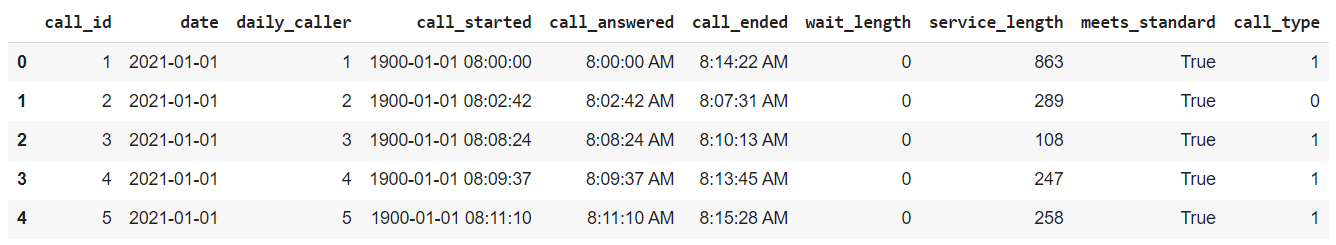
\includegraphics[scale= 0.6]{analise-de-dados/intro-analise/imgintro.png}
    \caption{Banco de dados - 5 primeiras chamadas}
    \label{fig: bd_img}
\end{figure}

Na Figura \ref*{fig: bd_img}, pode-se observar a estrutura da base de dados, assim como as colunas descritas a seguir:

\begin{itemize} 
    \item"call\_id" é a identificação da ligação (chave primária);
    \item"date"\;é a data da ligação;
    \item "daily\_caller"\;numera as ligações em um dia;
    \item"call\_started", "call\_answered" e "call\_ended"\;são os instantes de chegada, atendimento e término  da ligação, respectivamente;
    \item "wait\_length"\;é o tempo de espera;
    \item"service\_length"\;é o tempo de atendimento;
    \item"meets\_standard"\;retorna verdadeiro caso o tempo de espera seja menor do que um minuto;
    \item"call\_type" é o tipo da ligação.
\end{itemize}

Todos os tempos da base de dados estão em segundos.\\
Para os testes de hipóteses atrelados às diferenças entre essas variáveis em diferentes períodos foi utilizado o teste de Kolmogorov-Smirnov para duas amostras, que possui caráter não paramétrico, com as seguintes hipóteses:\\

\begin{center}
$H_0$ : As amostras seguem uma mesma distribuição de probabilidade\\
$H_A$ : As amostras seguem distribuições de probabilidade diferentes
\end{center}

Posteriormente à confirmação positiva da diferença entre amostras, foi realizado o teste de aderência das amostras às distribuições cauchy, chi quadrado, exponencial, gamma, lognormal, normal, powerlaw, rayleigh e uniforme.\\
Por fim, para analisar as correlações entre variáveis, foram realizadas regressões lineares e exponenciais.\\

\subsection{Ferramentas utilizadas}
A modelagem e as análises estatísticas do projeto foram realizadas utilizando a linguagem Python em sua versão 3.9, por meio do ambiente Google Colab.\\
Para isso, foram utilizadas as seguintes bibliotecas de Python:

\begin{itemize}
    \item Jupyter-notebook;
    \item Pandas;
    \item Numpy;
    \item Seaborn;
    \item Fitter;
    \item Scipy;
    \item Tabulate;
    \item Scikit-learn;
    \item Statsmodels;
    \item Matplotlib.
\end{itemize}